%%%%%%%%%%%%%%%%%%%%%%%%%%%%%%%%%%%%%%%%%
% Imperial Placement Report Template
% LaTeX Template
% Version 1.0 (28/06/16)
%%%%%%%%%%%%%%%%%%%%%%%%%%%%%%%%%%%%%%%%%
%----------------------------------------------------------------------------------------
%	PACKAGES AND OTHER DOCUMENT CONFIGURATIONS
%----------------------------------------------------------------------------------------

\documentclass[12pt,titlepage]{article}
\usepackage[english]{babel}
\usepackage[utf8x]{inputenc}
\usepackage{amsmath}
\usepackage{amsfonts}
\usepackage{graphicx}
\usepackage[colorinlistoftodos]{todonotes}
\usepackage[toc,page]{appendix}
\usepackage{fancyhdr}


\pagestyle{fancy}
\fancyhf{}
\fancyhead[L]{\textit{\nouppercase{\rightmark}}}
\fancyhead[R]{\thepage}

\setlength{\parindent}{0em}

\begin{document}

\begin{titlepage}

\newcommand{\HRule}{\rule{\linewidth}{0.5mm}} % Defines a new command for the horizontal lines, change thickness here
\setlength{\topmargin}{0in}
\center % Center everything on the page


%----------------------------------------------------------------------------------------
%	HEADING SECTIONS
%----------------------------------------------------------------------------------------

\textsc{\LARGE Imperial College London}\\[1.5cm] % Name of your university/college
\textsc{\Large Department of Computing}\\[0.5cm] % Major heading such as course name

%----------------------------------------------------------------------------------------
%	TITLE SECTION
%----------------------------------------------------------------------------------------

\HRule \\[0.4cm]
{ \huge \bfseries Drone Delivery Network Simulation on SpatialOS\\\textit{Interim Report}}\\[0.4cm] % Title of your document
\HRule \\[0.4cm]

%----------------------------------------------------------------------------------------
%	AUTHOR SECTION
%----------------------------------------------------------------------------------------

\begin{minipage}[t]{0.4\textwidth}
\begin{flushleft} \large
\emph{Author:}\\
Paul \textsc{Balaji} \\
\end{flushleft}
\end{minipage}
\begin{minipage}[t]{0.5\textwidth}
\begin{flushright} \large
\emph{Supervisor:} \\
Prof.~William \textsc{Knottenbelt}
\end{flushright}
\begin{flushright} \large
\emph{Second Marker:} \\
To.~Be \textsc{Decided}
\end{flushright}
\end{minipage}\\[1cm]

%----------------------------------------------------------------------------------------
%	DATE SECTION
%----------------------------------------------------------------------------------------

{\large \today}\\[0.5cm] % Date, change the \today to a set date if you want to be precise


\vfill % Fill the rest of the page with whitespace

\end{titlepage}

% \renewcommand{\abstractname}{\large Abstract}
% \begin{abstract}
% test post pls ignore
% \end{abstract}
%
% \renewcommand{\abstractname}{\large Acknowledgements}
% \begin{abstract}
% ack
% \end{abstract}

\newpage

\tableofcontents

\newpage

\section{Introduction}
Drone technology is becoming increasingly popular. Their agility and ability to be used remotely makes them ideal for a number of use cases in  numerous industries such as film, law enforcement, emergency services, agriculture and commercial delivery\cite{Koontz}. \\

Due to numerous advances in technology, drones are quickly advancing to the point where human input is no longer a necessity. This has led to many companies showing interest in integrating drones with their work in the coming years. \\

Although it may be an engineer's dream for a fully automated world, drones in particular are a harrowing reminder that there are real risks associated with them. There are already several incidents of drones crashing into planes and flying into areas they shouldn't, most notably near Heathrow airport\cite{BBCNews2017}. All of this provides motivation to introduce some form of autonomous air traffic control system to navigate these drones to their respective destinations in a safe manner.\\

However, prior work has been done on the routing and navigation aspect of such a system. In order for drones to truly take over more aspects of our lives, we must look at how they can provide a tangible cost-benefit to specific use-cases. There is no doubt that simply removing the human element can save costs drastically, and there is none more exciting a scenario than with deliveries. For example, Amazon stands to increase their margins considerably if they can successfully pull off their Prime Air initiative\cite{Welch2015}.

% delivery market stands to gain even more by optimising deliveries for profit / consider QoS

% the natural next step is to schedule / distribute the deliveries across network in addition to routing

% not advisable to test in production, so best port of call is to simulate

% many companies are investigating how to produce richer, meaningful simulations [cite improbable / SpatialOS]

% we have shown a new model of deliveries based on a QoS value curve

% show how net profit in a system changes depending on the type of scheduling mechanism used

\subsection{Autonomous Systems}
\subsection{Making Money}


%**********************************************%
\newpage
\section{Background}
We first provide an insight into drones, and the considerations to account for when applying them in day to day life. Additionally we summarise prior work completed by Imperial students on an autonomous air traffic control system. \\

We then continue to discuss modern delivery networks and introduce a mechanism by which economic value is prioritised. Finally, we give details about Improbable's SpatialOS and the reasoning for using this platform for the drone simulation.

\subsection{Drones}
As we have introduced, drones stand to be a revolutionary part of our lives as we welcome the new, incoming era of automation. However, to be practical there are a few key concepts one must understand to ensure that they remain a help and not a harm or hinderence to mankind.

\subsubsection{No Fly Zones}
No Fly Zones (which we will abbreviate as NFZs) are geographical areas where a drone is not allowed to enter or fly at any altitude. Examples of these may include Hyde Park, Buckingham Palace, airports and military locations. Typically these are static obstacles that will always remain a NFZ, however we could also consider cases when they could be created dynamically.\\

Suppose there was an issue of national security, it would be beneficial for the security and intelligence services to set up a temporary NFZ around areas where they deem a risk so that they can conduct their own operations without worry of external parties interfering with the situation.

\subsubsection{Manned Aviation}
Manned Aviation is any form of airborne transport with humans on board. This would include passenger jets, private jets, helicopters and other miscallaneous vechicles. For simulation purposes, we can consider these to have straight paths from a start to an end because relative to the zig-zagging of drones - they are effectively straight.

It is paramount to avoid collisions with manned aviation because there is a high risk of human calamity, in addition to the bad press and financial costs associated with such an air traffic incident.

\subsubsection{Other Drones}
Naturally we would want to make sure that we avoid colliding into other drones as well. In a perfect system, a single air traffic controller would have totalitarian dominance over all drones that take to the skies - however this is not \textit{Black Mirror} and we have to assume that there will always be drones that this system will not be able to control or predict. \\

Nonetheless, a system can ensure that it navigates drones under its control as best as it can, avoiding these external drones and other rogue drones that may be flying with the sole intention of causing problems to others.

\subsubsection{Toll Zones}
Toll Zones are geographical areas where a drone has to pay an extra fee to pass through at any altitude. It is a very similar idea to the one that led to Congestion Charges being applied to much of central London. By restricting certain areas only to those who are willing to pay the fee to use the airspace, it reduces the density of air traffic in a specific area. \\

These charges could also be used as an incentive to reduce pollution in the toll zone, and the additional revenue generated by the toll fees could be used towards the drone-related systems in place within the zone.

\subsection{Autonomous Air Traffic Control (AATC)}
\subsubsection{What is AATC?}
During the Autumn Term of the 2016-17 academic year, several students undertook a group project in association with Microsoft and Altitude Angel to produce an autonomous air traffic control system. The goal of the project was to safely navigate drones from their start to their end goals, whilst avoiding obstacles and taking the shortest possible path to minimise battery use.

\subsubsection{Technical Overview}
AATC has a simple client-server architecture, where drones connect to the REST service to send their telemetry information and goal waypoints every second. The server sends back direction recommendations to navigate the drone to its destination. \\

Because it would have been too expensive to trial the system on actual drones, a test bench was also implemented that would simulate the drones polling the server and responding to its recommendations. This test bench produced a set of simulation data, that is then available to view on the AATC visualiser\cite{Balaji2017a}.

\begin{figure}[!hbpt]
  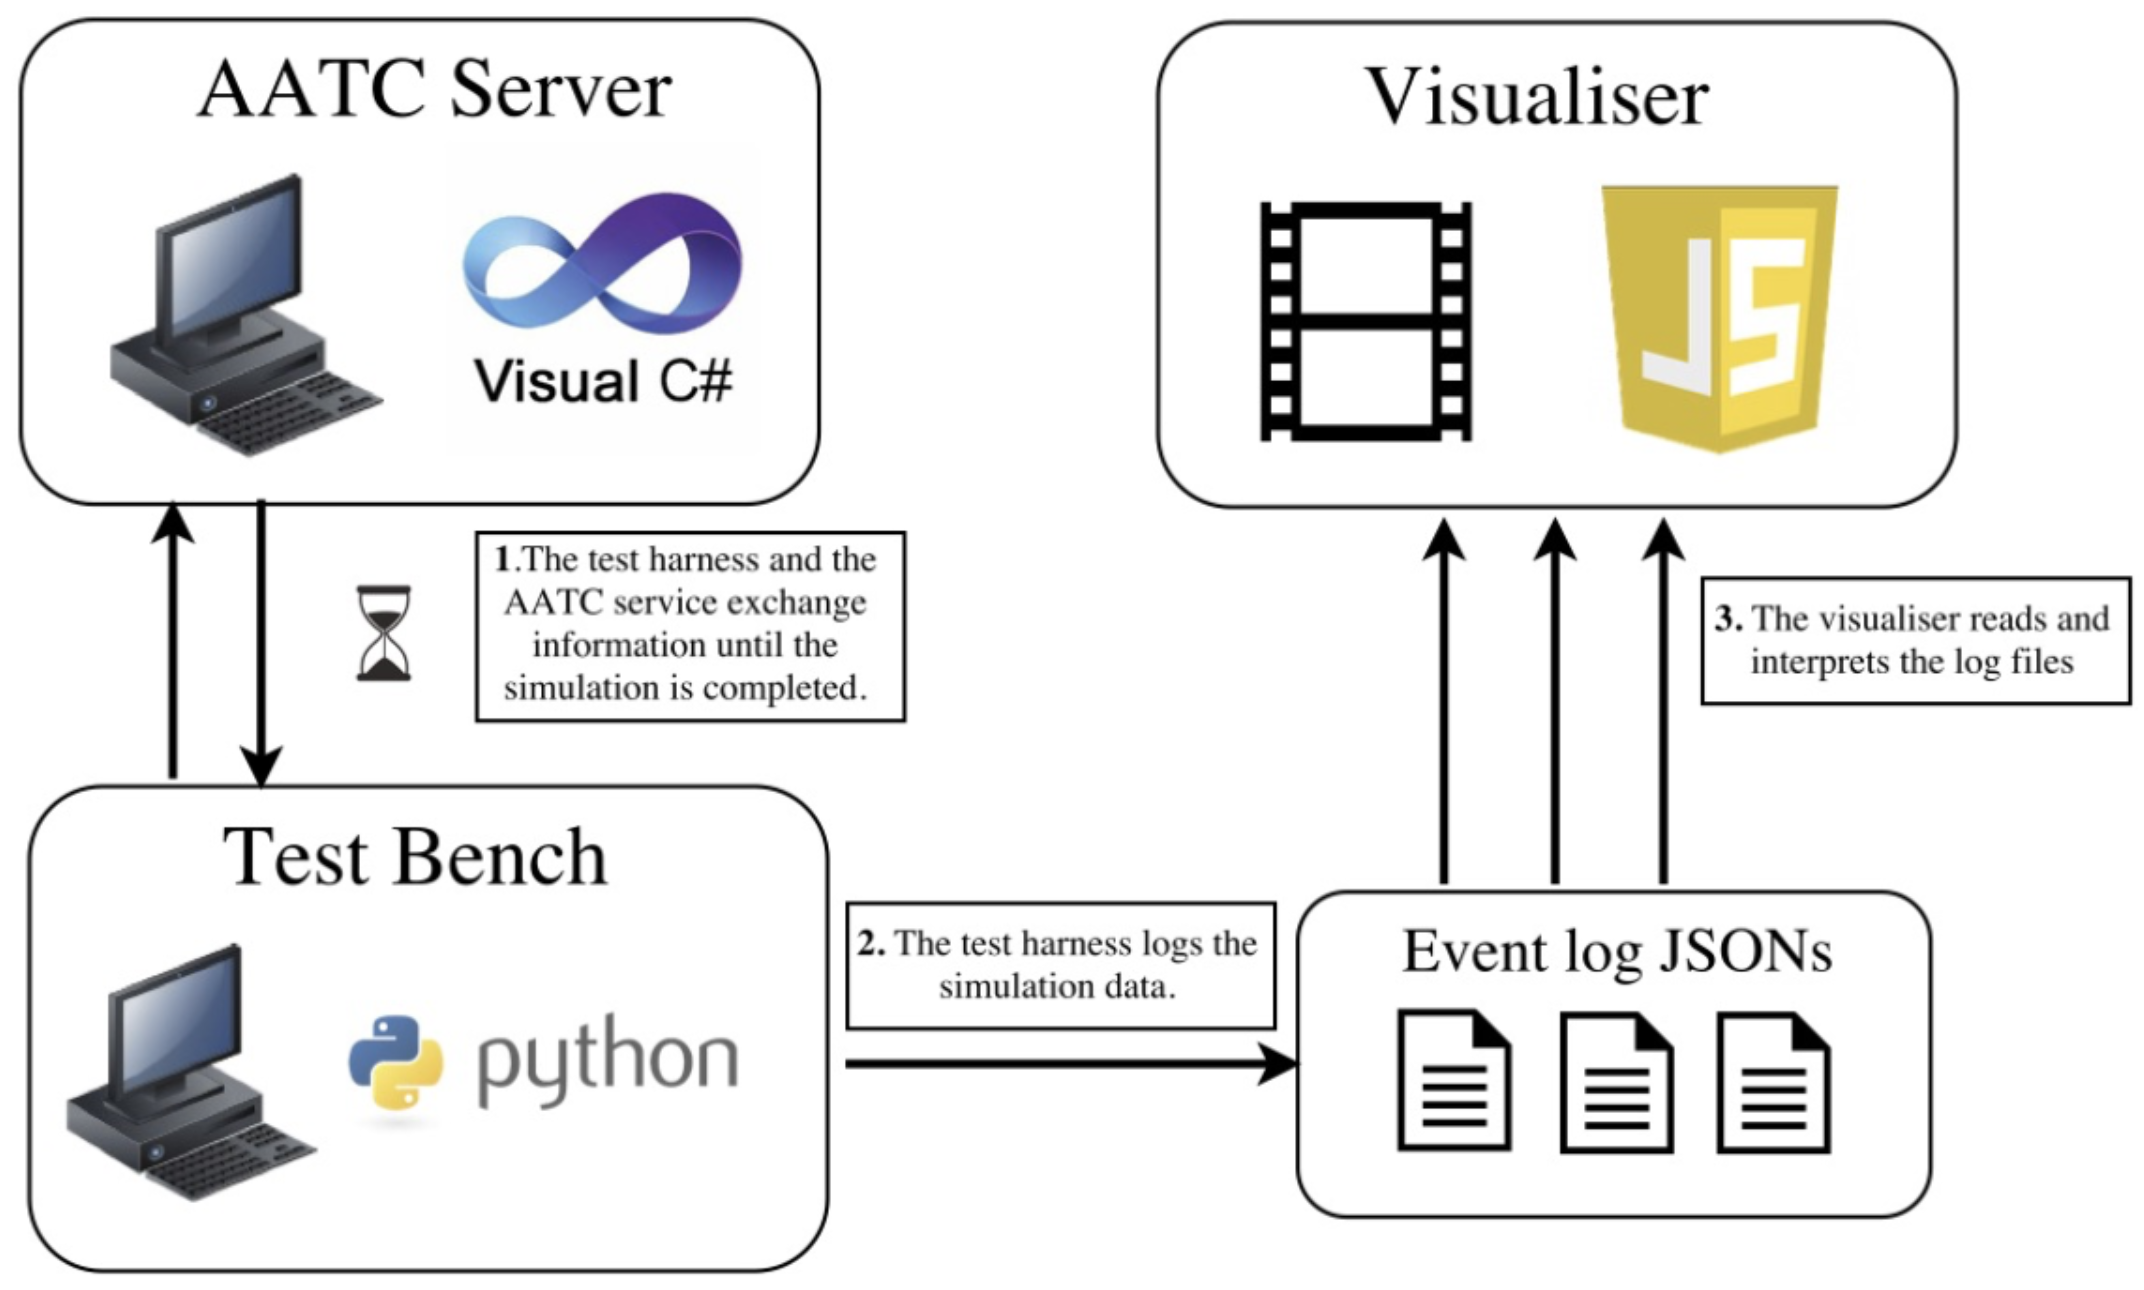
\includegraphics[width=\linewidth]{img/aatc_tech_overview.png}
  \caption{Technical Overview of AATC\cite{Balaji2017}.}
\end{figure}

The system was designed with three challenges in mind. The first challenge was to route drones from their origins to their destinations, and secondly, to ensure they avoided collisions with both static and dynamic obstacles - such as the ones mentioned in Section 2.1. The last challenge is to design the system in such a way that it would be able to scale to hundreds and thousands of drones.\\

To this end, a \textit{Global Layer} was built to deal with static obstacles (such as NFZs) by calculating a path for the drone around NFZs before it begins its journey. The second problem was tackled with a \textit{Reactive Layer} that handles non-static obstacles (such as manned aviation and other drones). This is the layer that would be providing the real-time updates to drones as they poll the server every second.

\subsubsection{Global Layer}
This layer holds the static representation of the world so that given a start and end, it can compute an optimal set of waypoints that a drone should follow.

\subsubsection{Reactive Layer}
This layer considers any dynamic obstacles that the drone may face, such as manned aviation, other drones and potentially dynamic NFZs.\\

Gobbledygoop


\subsubsection{Where to take it next?}

\subsection{Delivery Networks}
\subsubsection{Planes}
\subsubsection{Trucks}
\subsubsection{Drones}

\subsection{Prioritising Economic Value}
\subsubsection{Quality of Service}
\subsubsection{Value Curve}
\subsubsection{skdbsa}

\subsection{SpatialOS}
\subsubsection{Unity SDK}
\subsubsection{Layered Simulation}
\subsubsection{Distributed Simulation}
Example text 1\\

Example text 2\\

Example text 3

%**********************************************%
\newpage
\section{Project Plan}
\subsection{Phase 1: Porting Global and Reactive Layers to SpatialOS}
\subsection{Phase 2: Implementing a Scheduling Layer}
\subsection{Phase 3: Visualising the Economic Value}
\subsection{Stretch Goals}

%**********************************************%
\newpage
\section{Evaluation Plan}

%**********************************************%
%\newpage
%\section{Conclusion \& Future Work}
%blabla

%**********************************************%
\newpage
\addcontentsline{toc}{section}{References}

\bibliography{refs}
\bibliographystyle{abbrv}

\newpage

%\begin{appendices}
%\section{write something}
%The contents...
%\section{write something else}
%The contents...
%\end{appendices}

\end{document}
